% Options for packages loaded elsewhere
\PassOptionsToPackage{unicode}{hyperref}
\PassOptionsToPackage{hyphens}{url}
%
\documentclass[
]{article}
\usepackage{lmodern}
\usepackage{amssymb,amsmath}
\usepackage{ifxetex,ifluatex}
\ifnum 0\ifxetex 1\fi\ifluatex 1\fi=0 % if pdftex
  \usepackage[T1]{fontenc}
  \usepackage[utf8]{inputenc}
  \usepackage{textcomp} % provide euro and other symbols
\else % if luatex or xetex
  \usepackage{unicode-math}
  \defaultfontfeatures{Scale=MatchLowercase}
  \defaultfontfeatures[\rmfamily]{Ligatures=TeX,Scale=1}
\fi
% Use upquote if available, for straight quotes in verbatim environments
\IfFileExists{upquote.sty}{\usepackage{upquote}}{}
\IfFileExists{microtype.sty}{% use microtype if available
  \usepackage[]{microtype}
  \UseMicrotypeSet[protrusion]{basicmath} % disable protrusion for tt fonts
}{}
\makeatletter
\@ifundefined{KOMAClassName}{% if non-KOMA class
  \IfFileExists{parskip.sty}{%
    \usepackage{parskip}
  }{% else
    \setlength{\parindent}{0pt}
    \setlength{\parskip}{6pt plus 2pt minus 1pt}}
}{% if KOMA class
  \KOMAoptions{parskip=half}}
\makeatother
\usepackage{xcolor}
\IfFileExists{xurl.sty}{\usepackage{xurl}}{} % add URL line breaks if available
\IfFileExists{bookmark.sty}{\usepackage{bookmark}}{\usepackage{hyperref}}
\hypersetup{
  pdftitle={Flexible risk-based portfolio optimisation (Github link)},
  hidelinks,
  pdfcreator={LaTeX via pandoc}}
\urlstyle{same} % disable monospaced font for URLs
\usepackage[margin=1in]{geometry}
\usepackage{longtable,booktabs}
% Correct order of tables after \paragraph or \subparagraph
\usepackage{etoolbox}
\makeatletter
\patchcmd\longtable{\par}{\if@noskipsec\mbox{}\fi\par}{}{}
\makeatother
% Allow footnotes in longtable head/foot
\IfFileExists{footnotehyper.sty}{\usepackage{footnotehyper}}{\usepackage{footnote}}
\makesavenoteenv{longtable}
\usepackage{graphicx,grffile}
\makeatletter
\def\maxwidth{\ifdim\Gin@nat@width>\linewidth\linewidth\else\Gin@nat@width\fi}
\def\maxheight{\ifdim\Gin@nat@height>\textheight\textheight\else\Gin@nat@height\fi}
\makeatother
% Scale images if necessary, so that they will not overflow the page
% margins by default, and it is still possible to overwrite the defaults
% using explicit options in \includegraphics[width, height, ...]{}
\setkeys{Gin}{width=\maxwidth,height=\maxheight,keepaspectratio}
% Set default figure placement to htbp
\makeatletter
\def\fps@figure{htbp}
\makeatother
\setlength{\emergencystretch}{3em} % prevent overfull lines
\providecommand{\tightlist}{%
  \setlength{\itemsep}{0pt}\setlength{\parskip}{0pt}}
\setcounter{secnumdepth}{5}
\usepackage[]{natbib}
\bibliographystyle{plainnat}

\title{Flexible risk-based portfolio optimisation
\href{https://github.com/jhlandman/flex_rb_opt}{\emph{(Github link)}}}
\author{Emlyn Flint\footnote{Legae Peresec}, Jayson Landman\footnote{Ninety One Asset Management}}
\date{2020-07-05}

\begin{document}
\maketitle
\begin{abstract}
The purpose of this study is to present and test a general framework for risk-based investing. It permits various risk-based portfolios such as the global minimum variance, equal risk contribution and equal weight portfolios. The framework also allows for different estimation techniques to be used in finding the portfolios. The design of the study is to collate the existing research on risk-based investing, to analyse some modern methods to reduce estimation risk, to incorporate them in a single coherent framework, and to test the result with South African equity data. The techniques to reduce estimation risk draw from the usual mean-variance and risk-based optimisation literature. The techniques include regime switching, quantile regression, regularisation and subset resampling. In the South African experiment, risk-based portfolios materially outperformed the market weight portfolio out-of-sample using a Sharpe ratio measure. Additionally, the global minimum variance portfolio performed better than other risk-based portfolios. Given the long estimation window, no estimation techniques consistently outperformed the application of sample estimators only.

\textbf{Keywords}: risk-based investing, portfolio optimisaiton, estimation risk.
\end{abstract}

{
\setcounter{tocdepth}{2}
\tableofcontents
}
\hypertarget{about}{%
\section{About}\label{about}}

This is a research paper created with the \texttt{bookdown} package in R. It is intended to promote
reproducibility in academic research.

\hypertarget{introduction}{%
\section{Introduction}\label{introduction}}

If a risk-averse investor wants to construct portfolios with desirable properties, they would
ideally want to find allocations that offer an attractive risk-reward trade-off. \citet{M52} developed
modern portfolio theory and introduced the mean-variance optimal portfolio as a quantitative
solution to this asset allocation problem. However, the reward derived from this portfolio has to be
estimated from sample data and is often difficult to accurately predict - which, in turn, leads to
Markowitz's mean-variance portfolio being highly sensitive to the estimated portfolio inputs.

As an alternative, risk-based investing provides an avenue for finding portfolios for which expected
returns do not need to be estimated, and therefore resolves the portfolio expected return
sensitivity problem. Examples of risk-based portfolios commonly seen in practice are the global
minimum variance portfolio, the equal risk contribution portfolio, and the equal weight portfolio.
These three portfolios are optimal for investors that prioritise weight diversification, risk
diversification, or a specific combination of both.

Nevertheless, risk-based portfolios remain sensitive to covariance matrix estimation and hence
estimation risk. Improving risk-based estimation is done in three ways in this research. The first
improvement alters the covariance estimation procedure by accounting for differences in the sample
data. These changes include grouping to account for both non-normality and state-based
inhomogeneity. The second involves penalising the optimisation to limit the range of admissable
portfolios, which increases the investor's odds of choosing a well-estimated portfolio. The final
enhancement changes the implementation methodology entirely by performing the portfolio optimisation
on subsets of assets and then resampling to find an aggregate portfolio.

This research aims to bring together useful elements of risk-based portfolio estimation and
construction methodology into a single flexible framework. The general structure allows a choice of
risk-based portfolio as well as estimation risk reduction technique to improve the out-of-sample
portfolio performance. Once we have established a framework, the specific portfolio and estimation
technique, examples are developed theoretically. All of these reforms will be hollow without being
applied to actual financial data. Therefore, the various estimation techniques and risk-based
portfolio pairs are back-tested using South African equity data in an experiment, with the results
being measured by standard performance methodologies.

This research is built on the work of several different authors. Firstly - as with nearly all
portfolio construction research - this dissertation hinges on the modern portfolio theory of \citet{M52}.
It then considers the particular case of risk-based investing and makes use of the generalised
frameworks introduced by \citet{J13} and \citet{RR15}. Finally, in terms of improving the estimation and
optimisation processes, we make use of the ideas investigated by \citet{FD18}, \citet{K18}, and \citet{SW17}.

The rest of this dissertation is set out as follows. Chapter 2 outlines a general framework for
constructing risk-based portfolios and estimating them in a robust manner. Chapter 3 gives an
overview of the specific risk-based portfolios considered in this work. Chapter 4 presents several
techniques for reducing estimation risk, exploring their theoretical underpinnings and providing
general intuition. Chapter 5 then considers the empirical application of these techniques,
highlighting several technicalities. Chapter 6 then applies the flexible risk-based framework to SA
equity data, providing an empirical comparison of different implementations. Chapter 7 concludes the
research and provides avenues for further research.

\hypertarget{genframework}{%
\section{A framework for constructing risk-based portfolios}\label{genframework}}

\hypertarget{mpt}{%
\subsection{An overview of modern portfolio theory}\label{mpt}}

Every investor has a universe of \(N\) assets to which they can allocate capital. The proportion of
their allocation to the \emph{i}\(^{\text{th}}\) asset, \(w_i\), depends on the investor's risk and return
preferences. They could prefer riskier asset combinations because they require high capital growth,
or they could prefer more stable asset combinations that prioritise capital preservation. The column
vector \(w = [w_1,w_2,…,w_N]^\intercal\) is an \(N \times 1\) vector of allocations that define an
investor's portfolio. This portfolio is constrained by the investor's capital budget, which may be
articulated through the notion of weights. Therefore, all considered portfolios should adhere to the
budget constraint: \(\sum_i w_i = 1\).

In his seminal paper, \citet{M52} attempts to quantify the asset allocation process. Herein he posits that
the investor has to make a risk-reward trade-off when considering their portfolio returns,
\(R_\mathrm{p}\), over a pre-determined time horizon \([0, T]\). In his framework, he measures risk with
the variance of portfolio returns \(\mathbb{V}\mathrm{ar}[R_\mathrm{p}] = w^\intercal \Sigma w\),
where \(\Sigma\) is the \(N \times N\) asset return covariance matrix. Markowitz measures reward by the
expectation of portfolio returns \(\mathbb{E}[R_\mathrm{p}] = w^\intercal \mu\), where \(\mu\) is the
\(N \times 1\) vector of expected asset returns. If the investor fixes expected returns to a constant,
\(\mathbb{E}[R_\mathrm{p}] = c\), they encounter the problem of minimising portfolio risk,
\(\mathbb{V}\mathrm{ar}[R_\mathrm{p}]\). The mean-variance optimal (MVO) portfolio \(w_\mathrm{mvo}\)
achieves this goal while adhering to the budget constraint and the fixed expected return constraint.
Written mathematically, \(w_\mathrm{mvo}\) is the solution to the following Markowitz optimisation:
\begin{align} 
w_\mathrm{mvo} &= \underset{w}{\text{argmin}} \Big \{ w^\intercal \Sigma w \Big \},
\label{eq:mvoone}
\end{align}
subject to the constraints:
\begin{align*}
\mathcal{C}(w) &= 
\begin{cases}
 w^\intercal \mu &= c \;\;\;  \\
w^\intercal \underline{1} &= 1 \;\; .
\end{cases}
\end{align*}

There is a complication when using this framework in practice because \(\Sigma\) and \(\mu\) are
unknown. The investor can only observe a small set of sample returns from the underlying stock
processes that use these quantities as inputs. The sample returns, represented by a \(N \times T\)
matrix \(\textbf{X}\), can be used to estimate \(\Sigma\) and \(\mu\). The sample estimates are:

\begin{align}
\textbf{S}&=  \frac{1}{T - 1}(\textbf{X} - \mathbf{\bar{x}} \underline{1}^\intercal_T)(\textbf{X} - \mathbf{\bar{x}} \underline{1}^\intercal_T)^\intercal, \label{eq:samplevar} \\
\mathbf{\hat{\mu}} &= \mathbf{\bar{x}} , \label{eq:samplemean}
\end{align}
where \(\mathbf{\bar{x}}\) is a \(N \times 1\) vector of mean returns. A total of \(\frac{N(N+1)}{2}\)
distinct parameters are being estimated for the sample covariance matrix (SCM) while \(N\) distinct
sample expected returns are estimated. \(\textbf{S}\) and \(\hat{\mu}\) can be substituted into
equation \eqref{eq:mvoone} to infer an MVO portfolio, \(\hat{w}_\mathrm{mvo}\). For each level of
portfolio return \(c = \hat{w}^\intercal \hat{\mu}\), an estimated portfolio volatility level
\(\mathbb{SD}[\hat{R}_\mathrm{p}] = \sqrt{\hat{w}^\intercal\textbf{S}\hat{w}}\) is realised. These
estimated expected return-volatility pairs induce a frontier in the expected return-volatility
plane, which may or may not be close to the frontier implied by the actual inputs \(\Sigma\) and
\(\mu\). The actual frontier is optimal for the Markowitz framework, and he terms it the `efficient
frontier'.

The above framework and estimation procedure yields a solution to the asset allocation dilemma, but
there is still a sensitivity predicament. \citet{M89} shows that the MVO procedure, as described above,
overweights assets with substantial estimated returns \(\mathbf{\bar{x}}\). However, these are the
same assets that are likely to have been misestimated. Thus, any potential estimation errors are
`maximised' - an undesirable property that makes \(\hat{w}_\mathrm{mvo}\) a potential liability for
the investor to hold.

The MVO procedure is commonly adjusted to reduce sensitivity to the input \(\mathbf{\bar{x}}\) in one
of two ways. The first is to estimate expected returns in a manner that targets return drivers or
factors, which has motivated the rise of factor-based investing \citep{A14}. The second adjustment is to
remove the dependency on expected return estimates altogether and only construct portfolios based
on their risk properties. The latter has inspired the field of risk-based investing and is the
focus of this dissertation.

\hypertarget{introducing-risk-based-investing}{%
\subsection{Introducing risk-based investing}\label{introducing-risk-based-investing}}

A general risk-based portfolio optimisation programme is given below in equation \eqref{eq:rbintro}.
Removing the expected return constraint and altering the previous MVO optimisation problem for the
consideration of a generalised objective risk function \(f(\cdot| \textbf{X})\) yields:
\begin{align}
w^* = \underset{w}{\text{argmin}} \Big \{ f(w, \Sigma| \textbf{X}) \Big \}, \label{eq:rbintro}
\end{align}
subject to the constraint:
\begin{align*}
w^\intercal \underline{1} &= 1 \;\; ,
\end{align*}

where \(f(\cdot | \textbf{X})\) is a risk metric to be minimised. The choice of \(f(\cdot | \textbf{X})\) determines which risk-based portfolio is the optimal solution. Chapter \textbf{make
chapeter} expounds on the risk-based portfolio types relevant to this research.

The range of feasible portfolios given by equation \eqref{eq:rbintro} is practically too general
because unlikely single asset weights are still possible. To this end, an investor should apply a
weight constraint to limit feasible allocations, ensuring comparability with practical investing.
\citet{JM03} show that risk-based long-short portfolios can have extreme weights in practice, which are
unlikely to be accepted by an investor.

Additionally, \citet{JM03} also conclude that imposing the long-only investment constraint on US equities
leads to improved efficiency for optimal portfolios constructed with the first two sample moments
\(\hat{\mu}\) and \(\textbf{S}\). Hence, applying the long-only constraint is both statistically
appropriate and practically relevant for most investors.

Equally important is that an investor will be reluctant to concentrate their portfolio in a small
number of assets. Limiting the maximum single asset allocation to a selected weight \(\alpha\) avoids
such concentration. These constraints are concurrently expressed as
\(\{w :0 \leq w_i \leq \alpha, \; \forall i \}\) and can be added to optimisation \eqref{eq:rbintro}.
In its current form, the developed framework is still somewhat abstract, so it is not obvious how
to improve it. Even so, one can always define specific properties that the framework ought to have
for there to be a good chance of it operating as intended.

\hypertarget{improving-risk-based-portfolios}{%
\subsection{Improving risk-based portfolios}\label{improving-risk-based-portfolios}}

\citet{H23} defines a mathematical problem as `well-posed' if:

\begin{enumerate}
\def\labelenumi{\arabic{enumi}.}
\tightlist
\item
  the solution exists,
\item
  the solution is unique,
\item
  the solution is not overly sensitive to small perturbations in inputs.
\end{enumerate}

Well-posed problems are easier to work with and are more stable than ill-posed problems - ones that
fall short of the definition. The expected return constraint was previously disregarded for MVO
portfolios because the MVO framework often does not meet requirement 3. when the sample mean returns
estimate \(\mu\). Risk-based portfolios are therefore more `well-posed' than MVO portfolios.

However, there are two common ways in which risk-based portfolios are also ill-posed. The first is if
there are very few sample observations; namely, if \(T < N\). In this scenario, the covariance matrix
is not of full rank and is therefore not invertible, causing non-unique solutions to \(w^*\). The
framework is then ill-posed by 2. The second is if small changes in \(\textbf{X}\) result in large
deviations of \(w^*\). The framework is then ill-posed by 3. Many researchers such as \citet{JK81}
and \citet{B91} have shown that the latter phenomenon is observed in practice, and often persists even
if \(T\) is much larger than \(N\). To address point (iii) and make the problem well-posed, one needs a
measure of sensitivity. We outline a pseudo-derivation of a sensitivity measure below.

\citet{K18} views the portfolio optimisation problem from a modelling perspective. The returns on the
portfolio are modelled directly by an unknown function \(g(\cdot)\):
\begin{align}
R_p & = g(\textbf{X}) + \epsilon, \label{eq:retmodel}
\end{align}
where \(\epsilon\) has the normal distribution with zero mean and variance \(\phi^2\). Estimating
\(g(\cdot)\) is the aim of using the framework, and it is a real-valued function that is not
necessarily differentiable or continuous. Each algorithm \(q\) refers to a combination of estimation
procedure for the inputs, and a computation of a risk-based portfolio using equation
\eqref{eq:retmodel}. Each \(q\) specifies an estimate of the function \(g\), denoted \(\hat{g}_q\). In the
same way that \(\hat{w}^*\) (\(w^*\) calculated with sample inputs \(\textbf{S}\) and \(\hat{\mu}\)) can be
used to estimate the out-of-sample risk-based portfolio, \(\hat{g}_q\) can predict out-of-sample
portfolio returns, which are forecasted most accurately by the unobservable function \(g\).

It is necessary to distinguish between the two types of data that are available. The first is
historical data comprising of the matrix \(\textbf{X}_0\) and in-sample returns \(R_{\mathrm{p}, 0}\),
which combine to form the set \(\mathcal{H}_0\). The second is out-of-sample data \(\textbf{X}_1\) and
\(R_\mathrm{p, 1}\), which combine to form the set \(\mathcal{H}_1\). Algorithm \(q\) does not utilise the
data contained in \(\mathcal{H}_1\), which are chronologically realised after the most recent points in
\(\mathcal{H}_0\). A mean squared error penalty is appropriate to measure the accuracy with which
\(\hat{g}_q (\textbf{X}_1)\) (estimated using \(\mathcal{H}_0\)) predicts the out of sample returns
\(R_\mathrm{p, 1}\). \citet{K18} terms the expectation of the out-of-sample mean squared error
``generalisation error'' (GE), shown mathematically as:
\begin{align}
GE(\hat{g}_q) & = \mathbb{E}[(R_\mathrm{p, 1} - \hat{g}_q (\textbf{X}_1))^2|{\mathcal{H}_1}],
\end{align}
where GE is specific to a sample. The actual quantity of interest is the expected performance of \(q\)
for many potential sample sets, as we are evaluating \(q\)'s efficacy holistically. This quantity is
called the expected generalisation error across all samples, denoted \(G_q\). Furthermore, \(G_q\) may be
decomposed \footnote{The decomposition is shown by \citet{FHT01}.} to reflect a common modelling trade-off between
bias and variance:
\begin{align}
G_q &:= \mathbb{E} \Big [ \mathbb{E}[(R_\mathrm{p, 1} - \hat{g}_q (\textbf{X}_1))^2|{\mathcal{H}_1}] \Big | \mathcal{H}_0\Big ] , \\
& = \underbrace{ \Big (g(\textbf{X}_1) - \mathbb{E}[\hat{g}_q (\textbf{X}_1)|\mathcal{H}_0] \Big )^2}_{\text{squared bias}} + \underbrace{\mathbb{V}\mathrm{ar} [\hat{g}_q(\textbf{X}_1)|\mathcal{H}_0]}_{\text{variance}} + \underbrace{\phi^2}_{\text{irreducible error}}.\label{eq:bvdecomp}
\end{align}
The squared bias is the extent to which the expectation of predicted returns differs from the best
possible predictor of returns, the correct function \(g(\cdot)\). The variance measures the magnitude
by which the predicted returns will vary under repeated sampling. By setting
\(\hat{g}_q(\cdot) = g(\cdot)\) in equation \eqref{eq:bvdecomp} only statistical noise remains; hence,
the noise is irreducible. The risk of misestimating \(g(\cdot)\) should not include the risk that is
retained by even the best estimator. Therefore, estimation risk is considered as the sum of the first
two terms only, the squared bias and the variance. An over-fitted algorithm will have high variation
for repeated samples. An under-fitted algorithm will have high bias and be consistently poor for
repeated samples. The over- and under-fitting trade-off is an example of how the bias-variance
trade-off works in practice.

Until now, we have assumed that the estimated portfolio \(\hat{w}^*\) from equation \eqref{eq:rbintro}
is an unbiased estimate of the actual risk metric-minimising portfolio \(w^*\) because the choice of
\(f(\cdot | \textbf{X})\) determines precisely the type of risk-based portfolio. However,
\(f(\cdot|\textbf{X})\) does not precisely determine the estimation risk. Employing a penalty on the
objective function introduces bias to reduce estimation risk, \emph{i.e.} hopefully, the squared
bias increase does not outweigh the variance decrease. The introduction of the penalty yields an
estimated portfolio \(\hat{w}^*\) that is consistently closer to \(w^*\) than an unbiased portfolio would
be. The penalty constraint can be stated as \(P(w) \leq s\) and reduces the set of all possible
portfolios. If done correctly allocations that are misestimated by the heftiest margins are excluded
by this constraint, and allocations that are consistently closer to the actual portfolio remain. The
general risk-based framework can now be restated as below to accommodate the penalty using a
Lagrangian multiplier approach:
\begin{align}
w^* = \underset{w}{\text{argmin}} \Big \{ f(w, \Sigma| \textbf{X}) + \lambda P(w) \Big \}, \label{eq:genopt}
\end{align}
subject to the constraints:
\begin{align*}
\mathcal{C}(w) &= 
\begin{cases}
w^\intercal \underline{1} = 1 \;\; \\
0 \leq w_i \leq \alpha, \; \forall i \;\;\; ,
\end{cases}
\end{align*}

where \(P(\cdot)\) is the penalty function, and \(\lambda\) is the Lagrangian multiplier. Kinn proposes
estimating \(\lambda\) in a way that is consistent with the rest of the optimisation. Therefore, we
apply the \(\lambda\) estimation that minimises the portfolio specific risk metric using in-sample
data. Additionally, by setting \(\lambda = 0\), the unpenalised portfolio can still be recovered.
Optimisation \eqref{eq:genopt} will be the general risk-based portfolio optimisation going forward.

Improving on the vanilla risk-based optimisation is done in three ways in this research, and these
improvements are also common in the literature. Approach one deals with the assumption in equation
\eqref{eq:retmodel} that \(\epsilon\) has a normal distribution, and that the errors through time are
independent and identically distributed. If \(\hat{g}_q\) fails to approximate \(g\) correctly, then the
assumption is violated. There could be natural heterogeneity in the data accounted for by \(g\). \citet{FD18}
attempt to deal with heterogeneity by changing the estimation procedure of \({g}\) so that it includes
and accounts for potential differences in each observation of sample data. They do this through the
application of regimes and quantiles, grouping the input data to increase the accuracy of the
estimated model. The second approach adapted from \citet{K18} has already been shown above and
involves penalising the optimisation and setting \(\lambda > 0\) in equation \eqref{eq:genopt}. The
third and final approach requires resampling from the observations in \(\textbf{X}\) for different
subsets of assets and hinges on implementation adjustments. \citet{SW17} suggest finding \(w^*\)
multiple times for different resampled subsets and blending the result afterwards to find an
aggregate weight, that hopefully reduces estimation risk. Chapter \textbf{insert chapter ref} contains a
more detailed exploration of these techniques. Before that, further investigation of desirable risk
properties and the portfolios that have them is required to specify \(f(\cdot|\textbf{X})\).

\hypertarget{rbportch}{%
\section{Overview of risk-based portfolios}\label{rbportch}}

There are many types of risk-based portfolios, for a broader analysis refer to \citet{DV17}. In this chapter,
we review three risk-based portfolios: the global minimum variance, equal weight and equal risk
contribution portfolios. The risk properties that these portfolios have, the strategies that bear them
out and the conditions under which they perform optimally are all covered.

\hypertarget{risk-based-portfolio-types}{%
\subsection{Risk-based portfolio types}\label{risk-based-portfolio-types}}

Each risk-based portfolio is optimal in some sense because they all minimise a specific objective risk
function. The nature of the objective function depends on the investor's risk preferences. In line
with \citet{M52}, a genetic risk metric to minimise is the portfolio variance, as an investor may not be
willing to tolerate large swings in capital value. Setting
\(f(\cdot|\textbf{X}) = w^\intercal \Sigma w\) in portfolio optimisation \eqref{eq:genopt} yields the
global minimum variance (GMV) portfolio, denoted \(w_\textrm{gmv}\). The objective function is the same
as for the MVO portfolio for an imputed value of \(c\), meaning that the GMV portfolio sits on the
efficient frontier. The GMV portfolio is also the only risk-based portfolio that is always on the
efficient frontier.

\citet{MRT10} utilise the concept of an asset's marginal risk contribution (MRC) in a portfolio to perform
risk-based portfolio calculations. It is the sensitivity of the portfolio volatility to the weight of
an asset in a portfolio. Alternative representations of the MRC and an outline of why the weighted sum
of the MRC's is minimised for the GMV portfolio are shown in appendix \textbf{insert appendix ref}. Below
is the mathematical definition of the MRC for the \(i^{\mathrm{th}}\) asset:
\begin{align}
\frac{\partial}{\partial w_i} \Big [ \sigma(w) \Big ]= \frac{(\Sigma w)_i}{\sqrt{w^\intercal \Sigma w}}.
\end{align}

When taking the realised portfolio returns as the single risk factor, there is no idiosyncratic risk
present for assets in the portfolio against this factor. Accordingly, the GMV portfolio is the lowest
possible beta portfolio. The GMV portfolio is, therefore, optimal for the investor that always takes
on the least risk at the margin. However, risk has to be estimated, so the investor only knows what
the least risky options available to them are in a historical sense. The downside is that always
choosing the lowest marginal risk contributing asset is implicitly displaying a high level of
confidence in estimations of risk.

Contrastingly, the investor may be at a loss when estimating risk. The only measure of diversification
for such an investor is weight diversification. To minimise their risk taken at the margin, this
investor would hold the smallest possible weight in each of the assets while still satisfying the
constraints. This strategy ensures that the investor avoids the maximum marginal risk contributing
asset to the greatest extent possible given that they are unsure which of the \(N\) assets it is. The
least weight concentrated portfolio that this strategy alludes to is the equal weight (EW) portfolio:

\begin{align}
w_{ew} & = \Big [\frac{1}{N} \; \cdot \cdot \cdot \frac{1}{N} \Big ]^\intercal \; ,
\end{align}

where the weight diversification measure that this portfolio maximises is the inverse Herfindahl index
(IHI), calculated as \(H^{-1} (w) = (\sum_{i = 1}^N w_i^2)^{-1}\). The most weight concentrated
portfolio is the single asset portfolio - where a single non-zero asset weight is \(1\). The IHI of this
portfolio is \(1\), which is as low as it can be. On the other hand, the EW portfolio has an IHI value
of \(N\). All portfolios, therefore, have an IHI on the interval \([1, N]\). In the presence of a maximum
weight constraint, the lower bound of the interval changes. The new lower bound is derived in appendix
\textbf{insert appendix ref}. To find the EW portfolio using framework \eqref{eq:genopt}, set the objective
function to the Herfindahl index, \(f(\cdot|\textbf{X}) = \sum_{i = 1}^N w_i^2\). No parameters in the
objective function require estimation, so this is a sample return independent optimisation, which
reflects the investor's lack of confidence in historical data.

The GMV and EW portfolios represent two extremes of investors, specifically those that value
volatility reduction only and those that value weight diversification only. The inequality
\(\sigma(w_{gmv}) \leq \sigma(w^\diamond) \leq \sigma(w_{ew})\) verifies this intuition. The portfolio
\(w^\diamond\) has intermediate weight concentration. Proof of the inequality is given in appendix
\textbf{insert appendix ref}. It is unlikely that a capital allocator will completely disregard one
risk-based approach for another. One method to construct a sound intermediate portfolio that
incorporates the MRC philosophy from the GMV portfolio construction and the high risk-asset avoidance
philosophy from the EW portfolio construction is to equalise the total risk contribution (TRC) from
each asset. An asset's TRC is the product of its MRC and its weight in the portfolio:
\begin{align*}
\text{TRC}_i &= w_i \cdot \frac{\partial}{\partial w_i} \Big [ \sigma(w)\Big ], \\
& = \frac{w_i \cdot (\Sigma w)_i}{\sqrt{w^\intercal \Sigma w}},
\end{align*}
where TRC's sum to the portfolio volatility. An equal risk contribution (ERC) portfolio equalises all
of the TRC's so that no single asset is a comparatively significant contributor to risk. The choice of
\(f(\cdot|\textbf{X})\) that minimises the squared distances between the TRC's to the greatest extent
possible is given below:
\begin{align}
f(w, \Sigma|\textbf{X}) &= \sum_{i = 1}^N  \sum_{j \geq i}^N(w_i(\Sigma w)_i - w_j(\Sigma w)_j)^2 \;\;  .
\end{align}

\citet{MRT10} show that a log-constraint on the weights in GMV optimisation could equivalently express this
choice of \(f(\cdot| \textbf{X})\) - an idea explored further in appendix \textbf{insert appendix ref}.
Therein it is shown that the ERC portfolio is an intermediate portfolio \(w^\diamond\). While there are
several other risk-based portfolios that have been suggested in the literature, we will focus our
attention only on these three portfolios, which are arguably some of the most common risk-based
portfolios seen in practice \citet{J13}.

\hypertarget{risk-based-portfolio-properties}{%
\subsection{Risk-based portfolio properties}\label{risk-based-portfolio-properties}}

Section \ref{mpt} introduces the Markowitz efficient frontier.@S64 extends this work to deduce that
there is an optimal portfolio called the tangency portfolio. He does make certain assumptions about
investors' preferences and the presence of a risk-free asset. The market-weighted (MW) portfolio is the
portfolio for which the efficient frontier is tangential to the line bisecting the y-axis at the
risk-free rate (\(r_\mathrm{f}\)) in the expected return-volatility plane. The MW portfolio is the
portfolio held by all investors in the market on average and is relevant because it offers the investor
diversification with negligible transaction costs \citet{P07}. The MW portfolio is not risk-based in the
traditional sense, but it does not require an estimate of expected returns to calculate; hence, the MW
portfolio offers a cheap benchmark against which to compare risk-based portfolio performance. However,
the holder of the MW does implicitly adopt all investors' weighted expectations of expected returns
\citet{H91}. The tangency portfolio is optimal for the Sharpe ratio (SR) measure under Sharpe's
assumptions. The measure is defined as:
\begin{align}
\text{SR}_\mathrm{p} = \frac{\mathbb{E}[R_\mathrm{p}] - r_\mathrm{f}}{\mathbb{SD}[R_\mathrm{p}]} \;.
\end{align}

Within the MVO construction, the MW portfolio has the maximum Sharpe ratio (MSR) and is, therefore, the
MSR portfolio. \citet{S07} shows that the MSR portfolio, \(w_\mathrm{msr}\), can alternatively be expressed
as the portfolio for which marginal excess returns and the MRC's are equal for all portfolio
constituents. \citet{J13} use this fact to find MSR optimality conditions for each of the risk-based
portfolios, some examples of which are shown in appendix \textbf{insert appendix num}.

Table \ref{tab:rbportprops} summarises the salient risk properties of the EW, ERC, and GMV
portfolios. Included is the strategy to find the portfolio, the requirements for when the portfolio
coincides with the MSR portfolio, and their empirical risk characteristics. The risk characteristics
entail whether the risk is inherent to the investment, the construction of the portfolio, or liquidity
restrictions when creating the portfolio.

\begin{longtable}[]{@{}llll@{}}
\caption{\label{tab:rbportprops} Risk-based investing portfolio properties \citet{J13}}\tabularnewline
\toprule
\begin{minipage}[b]{0.06\columnwidth}\raggedright
Portfolio\strut
\end{minipage} & \begin{minipage}[b]{0.09\columnwidth}\raggedright
Strategy\strut
\end{minipage} & \begin{minipage}[b]{0.39\columnwidth}\raggedright
MSR conditions\strut
\end{minipage} & \begin{minipage}[b]{0.34\columnwidth}\raggedright
Risk characteristics\strut
\end{minipage}\tabularnewline
\midrule
\endfirsthead
\toprule
\begin{minipage}[b]{0.06\columnwidth}\raggedright
Portfolio\strut
\end{minipage} & \begin{minipage}[b]{0.09\columnwidth}\raggedright
Strategy\strut
\end{minipage} & \begin{minipage}[b]{0.39\columnwidth}\raggedright
MSR conditions\strut
\end{minipage} & \begin{minipage}[b]{0.34\columnwidth}\raggedright
Risk characteristics\strut
\end{minipage}\tabularnewline
\midrule
\endhead
\begin{minipage}[t]{0.06\columnwidth}\raggedright
EW\strut
\end{minipage} & \begin{minipage}[t]{0.09\columnwidth}\raggedright
Equalise \(w_i\)\strut
\end{minipage} & \begin{minipage}[t]{0.39\columnwidth}\raggedright
Identical excess returns. Identical volatilities. Identical correlations.\strut
\end{minipage} & \begin{minipage}[t]{0.34\columnwidth}\raggedright
Medium to high risk. Insensitive to \(\Sigma\). Low turnover.\strut
\end{minipage}\tabularnewline
\begin{minipage}[t]{0.06\columnwidth}\raggedright
ERC\strut
\end{minipage} & \begin{minipage}[t]{0.09\columnwidth}\raggedright
Equalise \(TRC_i\)\strut
\end{minipage} & \begin{minipage}[t]{0.39\columnwidth}\raggedright
Identical Sharpe ratios. Identical correlations.\strut
\end{minipage} & \begin{minipage}[t]{0.34\columnwidth}\raggedright
Medium risk. Moderately sensitive to \(\Sigma\). Medium turnover.\strut
\end{minipage}\tabularnewline
\begin{minipage}[t]{0.06\columnwidth}\raggedright
GMV\strut
\end{minipage} & \begin{minipage}[t]{0.09\columnwidth}\raggedright
Equalise \(MRC_i\)\strut
\end{minipage} & \begin{minipage}[t]{0.39\columnwidth}\raggedright
Identical excess returns.\strut
\end{minipage} & \begin{minipage}[t]{0.34\columnwidth}\raggedright
Lowest risk. Highly sensitive to \(\Sigma\). High turnover.\strut
\end{minipage}\tabularnewline
\bottomrule
\end{longtable}

While the MSR conditions are theoretically compelling, out-of-sample optimality is harder to determine
in practice. \citet{H91} show that portfolios that are superior to the MW portfolio exist when:
short-selling is restricted, investments are taxed, and foreign investors are active market
participants. These portfolios should have the same expected return as the MW portfolio with lower
volatility. Their statement is true even in an `efficient market'. Studies of the historical
performance show that some portfolios outperform others. In these studies, the authors restrict the
asset universe to US equities; hence, their results will not necessarily translate to South Africa.
The hope of introducing risk-based portfolios is to find Haugen and Baker's superior portfolios.
Evidence supporting this ambition exists. \citet{DGL07} demonstrate the robust out-of-sample
performance of EW portfolios when compared to MVO and MW portfolios for a broad range of asset
universes. \citet{C06} also demonstrate that GMV portfolios show outperformance against the MW and MVO
benchmarks. They initially attribute this to the diachronic persistence of covariances when compared
to expected returns. In a later paper, \citet{C11} suggest that the outperformance is due to a bias
inherent in the portfolio construction towards stocks that do not move with the rest of the market,
but that still have comparatively high expected returns.

Within risk-based portfolios, \citet{K10} have shown that GMV portfolios outperform EW portfolios when the
implementer uses a long enough estimation window. Therefore, they establish a defence for using
optimisation on a sample covariance matrix. This research remains consistent with these findings,
using the EW portfolio as a benchmark in pursuit of better out-of-sample performance within the GMV
and ERC frameworks. In the next chapter, we outline the techniques used to achieve this aim.

\hypertarget{estimation-risk-reduction-techniques}{%
\section{Estimation risk reduction techniques}\label{estimation-risk-reduction-techniques}}

As stated in chapter \ref{genframework}, estimation risk is comprised of squared bias and variance.
There are many methods to approach reducing estimation risk, but in this research, we introduce three
ways that are consistent with the general risk-based investing framework presented in equation
\eqref{eq:genopt}. The first method deals with improving the estimation of the inputs to the risk-based
portfolio function \(f(w, \Sigma|\textbf{X})\), accounting for heterogeneity in the input data. The
second method involves penalising the optimisation objective function to obtain a portfolio estimate
with consistently lower deviation from the actual out-of-sample risk-based portfolio solution. The
final process entails changing the implementation method in a manner that reduces estimation risk.
Every risk reduction technique falls into one of these three categories.

\hypertarget{improving-optimisation-inputs}{%
\subsection{Improving optimisation inputs}\label{improving-optimisation-inputs}}

The first approach to improving on the sample ERC and GMV portfolios involves finding better estimates
for the input \(\Sigma\), given the set of sample returns. As stated in equation \eqref{eq:retmodel},
the function \(g\) deals with the sample returns in a manner that ensures the irreducible error,
\(\phi^2\), is independent and identically normally distributed. However, because \(g\) is unobservable,
our estimation \(\hat{g}\) might not ensure this property. Heterogeneity of sample errors for investment
portfolios has been observed in empirical finance by \citet{AC02}, who demonstrate that negative stock
price correlations are less pronounced in downward markets. Therefore, empirical finance suggests two
states of the world, one where the market is in turmoil, and one where the market is not.

\citet{K12} use these two states to determine separate multi-asset allocations for `turbulent' and `quiet'
markets and adopt a regime switching (RS) approach. To define two regimes, a metric to measure
turbulence is required. The authors take a squared Mahalanobis distance (SMD) approach to determine an
index through time. The Mahalanobis distance is a multi-dimensional generalisation of the notion of how
many standard deviations a point is away from the mean of a distribution. The SMD index (\(d_t\)) is
expressed mathematically as:
\begin{align}
d_t = (R_t - \mu)\Sigma^{-1}(R_t - \mu)^\intercal,
\end{align}
where: \[d_t = \mu_{s_t} + \sigma_{s_t}\epsilon_t,\] and \(\epsilon_t\) has a standard normal
distribution. The state at time \(t\) is shown by the random variable \(s_t\). As asserted earlier, the two
states are Quiet (\(Q\)) and Turbulent (\(T\)), hence \(s_t \in \{Q, T\}\). To calculate the SMD, we require
the unobservable inputs \(\Sigma\) and \(\mu\). They can be replaced by their sample counterparts,
\(\textbf{S}\) and \(\hat{\mu}\), to yield \(\hat{d}_t\). The SMD has a state-specific mean and volatility;
hence different values are observed based on the current system state. If the system emits large values
of \(\hat{d}_t\), the probability of being in a turbulent market is high. If the system emits small
values of \(\hat{d}_t\), the likelihood of being in a quiet market is high. The \(\zeta^{th}\) quantile of
the sample SMDs is the point where the system of reference changes. The market state is also an
unobservable variable, so the above model is referred to as a hidden Markov model (HMM). The HMM used
in this investigation is depicted in figure \ref{fig:hmm}.

\begin{figure}

{\centering 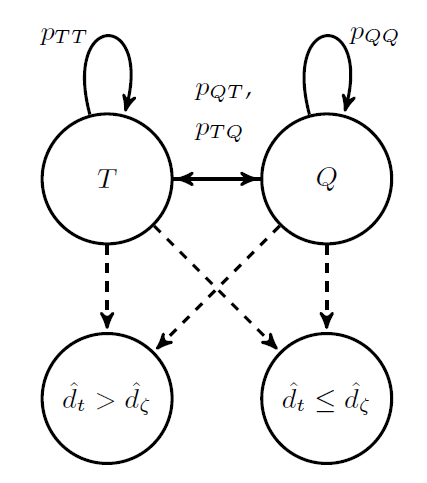
\includegraphics[width=5.93in]{quiet_turb_hmm} 

}

\caption{Turbulent / quiet hidden Markov model.}\label{fig:hmm}
\end{figure}

The transition matrix stores the probabilities of transition from a state at time \(t\) to another at
time \(t + 1\) for ease of computation. It is mathematically shown as:
\[P_{t, t + 1} = \begin{bmatrix} 
p_{QQ} & p_{QT} \\
p_{TQ} & p_{TT}  
\end{bmatrix},\]
where the matrix applies to all times \(t\). Because the matrix applies to all times the system is called
stationary, and the long-run probabilities of being in each state will converge. Once we have
determined the most likely state at time \(t\) using an algorithm such as the Viterbi algorithm, we can
use the series of estimated states \(\{\hat{s}_t: t \in \{0, 1, ..., T\}\}\) to partition the
data history. The two datasets would be data used for the quiet sample covariance matrix and data used
for the turbulent sample covariance matrix. \citet{FD18} blend these two sample matrices using the investor's
risk preferences and the most recent probabilities of being in each state, yielding a more
sophisticated estimator of \(\Sigma\).

An alternative approach to dealing with heterogeneity is to focus on the assumption that errors for
return forecasting models have a normal distribution. But first, we need to define a general return
forecasting model. If the return of a portfolio is viewed through a set of return drivers or risk
factors, then returns could be explained in part by those factors and the portfolio's sensitivity to
them. \citet{M10} encapsulates this idea in his asset return model given below:
\begin{align}
R &= \alpha +\beta^\intercal \mathcal{F} + \epsilon, \label{eq:retfact}
\end{align}
where \(R\) is a vector of asset returns (not portfolio returns through time as shown previously),
\(\alpha\) is a forecastable vector of returns unique to each security, \(\beta\) is a matrix of
sensitivities to risk factors, \(\mathcal{F}\) is a vector of factors, and \(\epsilon\) is the error
vector. The error vector is assumed to have a normal distribution. \citet{AC02} show that in a downward
market, the correlation structure is significantly different from what is implied by a normal
distribution, which is a problem when using model \eqref{eq:retfact} in the exhibited way. \citet{CDG19}
address the issue of non-normal errors by utilising the quantile regression model proposed by
\citet{KB78}. The asset returns, idiosyncratic asset returns, asset factor sensitivities and errors could all
be considered to be a function of the current quantile, denoted \(\tau\). This leads to the quantile
factor model (QFM):
\begin{align} 
\mathcal{Q}(\tau) =  \alpha(\tau) + \beta(\tau)\mathcal{F} + \epsilon(\tau), \label{eq:qfm}
\end{align}
where \(\tau \in [0, 1]\). In a different symmetric, normally distributed world, \(\tau\) can be set to
\(0.5\) and model \eqref{eq:retfact} will be recovered. However, in the real world where symmetry and
normality are often not adhered to, the quantile conditional errors can be defined more generally so
that they only have to satisfy:
\begin{align}
\mathbb{P}\Big[\epsilon(\tau) \leq \underline{0} \, \Big | \mathcal{F} \Big] = \tau \; .
\end{align}
This structure emerges from the cumulative distribution function (CDF) conditional on the set of
factors of each asset return \(R_i\). Given the conditional CDF for the returns on asset \(i\),
\(F_i(R_i|\mathcal{F})\), the quantile specific inverse CDF, \(F^{-1}_i(\tau| \mathcal{F})\), can be used
to generate the quantiles \(\mathcal{Q}_i(\tau)\). \citet{FD18} suggest using the information about each
quantile to construct a series of quantile-specific covariance matrices, which can then be blended to
yield a more sophisticated estimator of \(\Sigma\). Chapter \textbf{insert ref to next chapter} covers the
implementations of these two techniques to better estimate \(\Sigma\).

\hypertarget{penalising-the-optimization}{%
\subsection{Penalising the optimization}\label{penalising-the-optimization}}

To add a penalty term in a way that preserves the goal of the risk optimisation, we first need to
adapt the objective functions of each risk-based portfolio as given earlier in chapter
@ref\{rbportch\}. Consider the return-targeting penalised optimisation approach of \citet{K18}, both choices
of \(f(\cdot|\textbf{X})\) for the GMV and ERC portfolios can be adapted into this approach. Beginning
with the GMV portfolio, Kinn views the portfolio variance as an expectation:
\begin{align*}
f(w, \Sigma  | \textbf{X}) &= w^\intercal \Sigma w &\\
& = w^\intercal (\mathbb{E}[{r}_t {r}_t^\intercal] - \mu \mu^\intercal) w & \small\text{(alternate definition of $\Sigma$)} \\
& = \mathbb{E}[|w^\intercal \mu - w^\intercal {r}_t|^2],
\end{align*}
where \({r}_t\) represents the asset returns above the risk-free rate, and \(\mu\) is a vector of the
population expected excess returns as before. Rewriting the portfolio expected excess return as
\(\bar{r} = w^\intercal \mu\), the idea of return-targeting for a portfolio can be incorporated as the
expectation of \(|\bar{r} - w^\intercal {r}_t|^2\), which is the squared distance to a target return
level. Kinn's approach is consistent with an MVO optimisation intuitively because the target return
level is analogous an expected return constraint and minimising the return's squared distance to this
constraint is analogous to variance minimisation. The objective function can now be approximated using
the sample average as a result of the law of large numbers. We still have to show how to find the GMV
portfolio from an MVO procedure. As stated in table \ref{tab:rbportprops}, the GMV portfolio is the
MSR portfolio if the assumption of identical excess returns is met. Therefore, if the target return is
set to a value that is easily obtainable \(\bar{r} = \bar{r}_\mathrm{gmv}\), then the scheme will yield
a GMV portfolio. This easily obtainable value has to be found numerically and cannot be determined a
priori. The non-rigorous argument turns out to be empirically true for the portfolios analysed in this
research. When the return vector is replaced by the set of sample returns \(\textbf{X}\), and the
expectation is approximated by the sample average, the \citet{K18} form of objective function is recovered:
\begin{align}
f_{\text{Kinn}}(w|\textbf{X}) &= \frac{1}{T} \sum_{t = 1}^T  (\bar{r}_\mathrm{gmv} - \textbf{X}^\intercal_t w)^2, \label{eq:kinnop1}
\end{align}
where \(t\) indexes columns of the sample returns matrix \(\textbf{X}\). The GMV portfolio can be found equivalently in this way.

The log-constraint\footnote{The log-constraint is also introduced in appendix \textbf{insert appendix ref}.},
\(\sum_i \ln(w_i) \geq c\), can be placed on optimisation \eqref{eq:kinnop1} to recover the ERC
portfolio. To include the constraint in framework \eqref{eq:genopt}, a Lagrangian multiplier approach
can be used to move the log-constraint to the objective function. Kinn's adapted ERC objective
function is then:
\begin{align}
f_{\text{Kinn}}(w|\textbf{X}) &= \frac{1}{T} \sum_{t = 1}^T  (\bar{r}_{gmv} - \textbf{X}^\intercal_t w)^2 -\eta_{erc}\sum_{i = 1}^N \ln(w_i),
\end{align}
where \(\eta_{erc}\) is the Lagrangian multiplier scalar. Now that we have shown the standard objective
functions from earlier are equivalent to the Kinn framework, we have also vindicated the general
framework \eqref{eq:genopt} as accommodative of a valid application of supervised machine learning
(SML) to portfolio optimisation.

Because logical choices for \(f_{\text{Kinn}}(\cdot|\textbf{X})\) have been established, different
penalty functions can be applied to the optimisation. Two common penalised regression techniques are
lasso regression and ridge regression (RR). In the presence of a long-only constraint, as is applied
in this research, a lasso regression does not make sense, because the penalty function is simply the
sum of the absolute weights: \(P(w) = \sum_{i= 1}^N |w_i| =1\). This penalty is equal to \(1\) for all
constrained portfolios. Separately, the RR is obtained by specifying the penalty as the sum of squares
for the portfolio weights: \(P(w) = \sum_{i= 1}^N w_i^2\). The penalty reduces the number of admissable
concentrated portfolios and intuitively is not unlike incorporating some of the EW portfolio into the
ERC or GMV portfolios. Ignoring constraints, \citet{LW04} show that RR has the same effect as shrinking
the sample covariance matrix towards the identity matrix for the GMV optimisation:
\begin{align}
\textbf{S}_{RR} = \textbf{S} + \frac{\lambda}{T} \textbf{I}, 
\end{align}
where \(\lambda\) is the shrinkage intensity, and \(T\) is the number of sample observations. In the
presence of constraints, the actual scaling factor is slightly different from Ledoit and Wolf's
calculations, but the intuition of shrinkage towards the identity matrix still applies. If \(\lambda\)
becomes very large, the minimum variance portfolio will tend towards the EW portfolio. Estimating
lambda is thus a practical choice, and the process to do so consistently is outlined in the next
chapter.

\hypertarget{alternate-implementation-methods}{%
\subsection{Alternate implementation methods}\label{alternate-implementation-methods}}

\citet{SW17} present a means to find a resampled MVO portfolio that reduces estimation risk by optimising random subsets of assets in the investment universe. The process is called subset resampling (SRS). They then aggregate resultant optimised subset portfolios to create a final `optimal' solution. The procedure requires the inputs of a sample return matrix \(\textbf{X}\) and an asset subset size \(b\). The subset size is related to the extent of the trade-off between bias and variance. We have to choose the degree of repeated sampling, \(s\), which is restricted by the available computational power.

This method can be described as follows. For each of the \(s\) repeated samples, we randomly select the \(j^{\text{th}}\) subset of \(b\) assets from the \(N\) assets in the investment universe, denoted \(\mathcal{I}_j\). Using only the sample return data from the selected asset subset \(\textbf{X}_j\), we then compute the associated optimal portfolios \(\hat{w}_j\) using framework \eqref{eq:genopt} and a given choice of objective function. Finally, we average the \(s\) optimal subset weight vectors to obtain the final optimal asset portfolio \(\hat{w}_\mathrm{srs} = (\sum_{j = 1}^s \hat{w}_j)s^{-1}\).

The SRS process is very general, and could even be applied in conjunction with a penalised optimisation or an improved sample covariance matrix. Additionally, the user can choose the input \(b\). If \(b = N\), then the usual sample risk-based portfolio is recovered, albeit in a computationally expensive manner. If \(b = 1\), then the SRS procedure will yield the EW portfolio for a large enough value of \(s\). Therefore, \(b\) is the input parameter controlling the extent of the trade-off between weight diversification and estimation risk. The estimation of \(b\) should be done in a manner consistent with the aim of the optimisation. To ensure \(b\) scales with the size of the asset universe, \citet{SW17} recommend writing it in the form \(b = N^{\alpha}\), where \(\alpha \in [0, 1]\).

The SRS method is comparable to ensemble methods in machine learning. The logical basis is that many different models can be used and aggregated into a final model, rather than assuming a single model is the most accurate to use. Despite the general nature of the SRS procedure, it is still consistent with the approach of increasing the squared bias out of the hope that the variance reduction will offset it enough to lessen overall estimation risk.

Each of the three estimation risk reduction classes has at least one specific technique within them. Some modelling decisions need to be made for a prospective user to apply these techniques in an experiment. These modelling decisions are covered in the next chapter.

  \bibliography{biblio.bib}

\end{document}
